\documentclass[12pt]{report}

\usepackage{polski}
\usepackage[utf8]{inputenc}
\usepackage[unicode]{hyperref}

\usepackage{graphicx}
\graphicspath{ { . } }

\usepackage{url,apacite}
\bibliographystyle{apacite}


\title{Projektowanie i tworzenie stron i aplikacji webowych}
\date{06-01-2019}
\author{Kacper Karwot}

\begin{document}
 	\pagenumbering{gobble}
	\maketitle
	\tableofcontents
	\newpage
	\chapter{Wstęp}
	\section{Czym jest web development?}
	\textbf{Web development} to wszystkie zadania, które wchodzą w skład tworzenia strony sieci web, która może być dostępna w Internecie lub intranecie. 
	Web development to szerokie pojęcie, które może obejmować zarówno tworzenie prostej, statycznej strony zawierającej tekst lub 			skomplikowaną aplikację webową, usługę e-commerce lub serwis społecznościowy. 
 Wśród osób pracujących w branży, pojęcie "web development" zazwyczaj odnosi się do nie-projektowych aspektów budowania stron: tworzenia markupu i kodowania. Bardzo często używane są systemy zarządzania treścią(CMS) aby ułatwić dokonywanie zmian i pozwolić osobą mniej zaawansowanym technicznie na pracę nad stroną.
 	\newline
 	W większych organizacjach i biznesach, zespoły web developerskie mogą liczyć nawet setki osób i pracować według takich metodologii jak Agile podczas tworzenia produktu. Przy mniejszych projektach wystarczający może być jeden stały lub kontraktowy pracownik, ewentualnie pomocnicy specjalizujący się w grafice lub technicy IT. 
	\newline
	Wyróżniamy trzy rodzaje specjalizacji web developerów:
	\begin{itemize}
	\item[--] \textbf{front-end} developer,
	\item[--] \textbf{back-end} developer,
	\item[--] \textbf{full-stack} developer
 	\end{itemize}
 	
 	\cite{wiki:1}
 	
 	\newpage
	\section{Historia web developmentu}
	
	Tim Barners-Lee wynalazł World Wide Web w  1989, około 20 lat po pierwszym połączeniu, które dziś jest znane 
	jako Internet. Tim był inżynierem oprogramowania w CERN, gdzie dostrzegł potencjał wymiany danych naukowych przy pomocy
	milionów komputerów połączonych ze sobą za pomocą sieci.
	\newline
	W październiku 1990 sprecyzował trzy fundamentalne technologie, które do dziś są podstawą sieci
	\begin{itemize}
	\item \textbf{HTML} -(HyperText Markup Language) - pozwala formatować dokumenty oraz linkować inne dokumenty i źródła,
	\item \textbf{URI} - (Uniform Resource Identifier) - rodzaj ''adresu'' który jest unikalny dla każdego źródła w internecie,
	\item \textbf{HTTP} -(HyperText Transfer Protocol) - który możliwia pobieranie połączonych zasobów z całej sieci
	\end{itemize}
	
	W tamtym czasie Internet stał się prawdopodobnie najpotężniejszym narzędziem wymiany danych jakiego świat doświadczył. 
	\newline
	Tim Berners-Lee i inni zrozumieli, że aby sieć Web osiągnęła swój pełen potencjał, ich fundamentalne technologie muszą stać
	się światowym standardem, implementowanym w ten sam sposób na całym świecie. W ten sposób, w 1994 roku powstało
	\textbf{World Wide Web Consortium (W3c)} jako miejsce osiągnięcia konsensusu w sprawie specyfikacji i wytycznych, aby upewnić
	się, że sieć działa dla wszystkich i rozwija się w sposób odpowiedzialny.
	\newline
	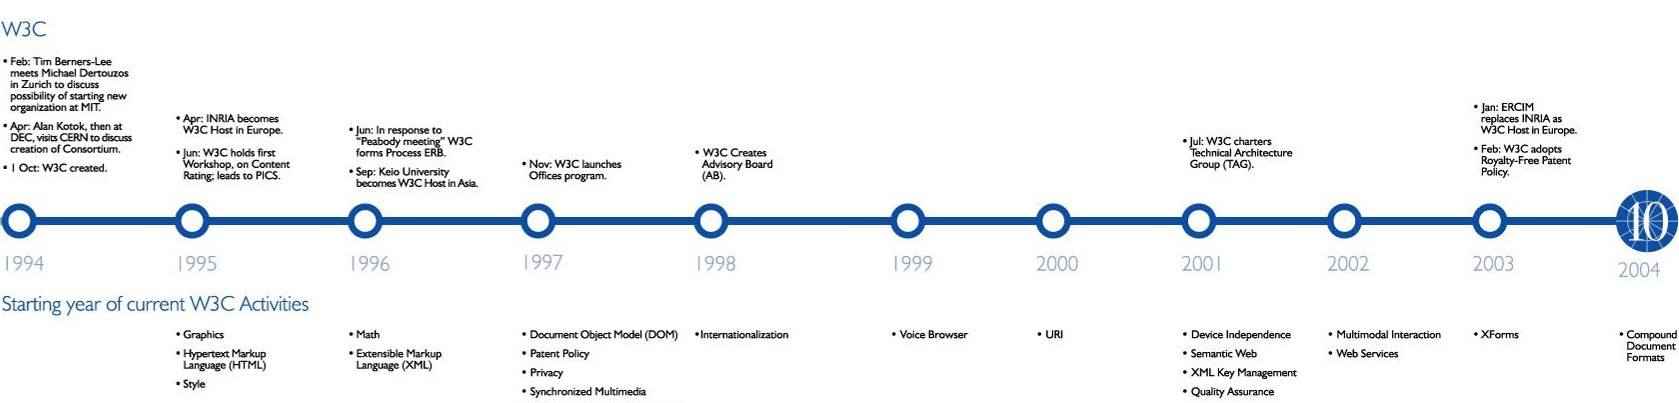
\includegraphics[width=\textwidth]{timeline.jpg}
	\newline
	\cite{history}
	
	\newpage 
	\chapter{Web development współcześnie}
	\section{Front-end}
	\newpage
	\section{Back-end}
	\newpage
	\section{Trendy w 2019 i 2020 roku}


	\newpage
	\chapter{Kim jest web developer?}
	\section{Kto może zostać web developerem?}
	\newpage
	\section{Czym zajmuje się web developer}

	\bibliography{b.bib}

\end{document}